\documentclass{sig-alternate}
%\documentclass{acm_proc_article-sp}
\usepackage{graphicx}
\usepackage{url}
\usepackage{paralist}
\usepackage{listings}
\usepackage{caption}
\usepackage{ntabbing}
\usepackage{tikz}
\usetikzlibrary{trees}

% \DeclareUnicodeCharacter{B1}{\pm}
%% LANGUAGE      Markup definitions
\def\lstxml{
  \lstset{language=XML,
    keywordstyle=\ttfamily,
    identifierstyle=\ttfamily\bfseries, 
    % commentstyle=\color{Brown},
    stringstyle=\ttfamily,
    showstringspaces=false,
    columns=[l]flexible, %% , basewidth={0.5em,0.4em}
    escapeinside={(@*}{*@)},
    morekeywords={encoding,
      mrow,math,mfrac,mi,msqrt,mo,mn,span,nobr,img}
  }
}

\def\lstjs{
  \lstset{language=Java,
    keywordstyle=\ttfamily,
    identifierstyle=\ttfamily\bfseries, 
    % commentstyle=\color{Brown},
    stringstyle=\ttfamily,
    showstringspaces=false,
    columns=[l]flexible, %% , basewidth={0.5em,0.4em}
    morekeywords={cvox,Api,Math,defineRule}
  }
}

\def\lsttex{
  \lstset{language={[LaTeX]TeX},
    texcsstyle=*\bfseries,
    keywordstyle=\ttfamily,
    identifierstyle=\ttfamily\bfseries, 
    % commentstyle=\color{Brown},
    stringstyle=\ttfamily,
    showstringspaces=false,
    columns=[l]flexible, %% , basewidth={0.5em,0.4em}
    moretexcs=intertext,
    morekeywords={sum,Sigma}
  }
}

\newcommand\ednote[1]{\typeout{There is still a note!!!}%
  {\bf EDNOTE: #1}}

\newcommand\edbf[1]{\typeout{There is still an editor's note!!!}%
  \textbf{EDNOTE: #1}}


\begin{document}
\title{Accessibility to Scientific Material:\\ The Case of Speaking Math}
\numberofauthors{2} %  in this sample file, there are a *total*

\author{
% You can go ahead and credit any number of authors here,
% e.g. one 'row of three' or two rows (consisting of one row of three
% and a second row of one, two or three).
%
% The command \alignauthor (no curly braces needed) should
% precede each author name, affiliation/snail-mail address and
% e-mail address. Additionally, tag each line of
% affiliation/address with \affaddr, and tag the
% e-mail address with \email.
%
% 1st. author
  \alignauthor Volker Sorge\titlenote{This work was done while the author spent a
    sabbatical at Google,
    Inc., Mountain View, CA, USA.}\\
  \affaddr{School of Computer Science}\\
  \affaddr{The University of Birmingham, UK}\\
  \email{V.Sorge@cs.bham.ac.uk}
% 2nd. author
\alignauthor
Charles Chen, T.V. Raman, David Tseng\\
       \affaddr{Google, Inc.}\\
       \affaddr{Mountain View, CA, USA}\\
       \email{\{clchen|raman|dtseng\}@google.com}
}


\maketitle 
\begin{abstract} 
  As the traditional methods of publishing and teaching in the
  STEM subjects are being progressively replaced by the provision
  of web-based content, ensuring full accessibility to this
  material for visually impaired users is of paramount importance
  for inclusive education. The text to speech translation of
  content for which well defined markup languages exists such as
  mathematics is a non-trivial problem. In this paper we present
  our efforts of making the speech translation of mathematical
  formulas a first class citizen in a general screen reader. We
  describe the ChromeVox screen reader and demonstrate how its
  features enable us to provide text to speech translation for
  web-based mathematical content. These features allow us to
  translate formulas given in a variety of formats into uniform
  spoken utterances exploiting ChromeVox's ability to handle
  alternative representations of DOM elements. This also allows
  us to customize aural rendering of mathematics both by using
  semantically enriched representations and employing flexible
  and adaptable speech rules. To further aid understanding of the
  math we exploit ChromeVox's idea of letting users engage with
  content on different levels of granularity to enable
  interactive exploration of complex mathematical formulas.
\end{abstract}
\category{H.5.2}{User Interfaces}{Voice I/O}
%A category including the fourth, optional field follows...
\category{H.5.4}{Hypertext}{Navigation, User Issues}

% \terms{}

\keywords{screen reader, mathematics, ChromeVox}

\section{Introduction}\label{sec:intro} 
Ensuring accessibility to scientific material has always been a challenging task
and can be considered a major obstacle for full inclusiveness in education in
the STEM subject, in particular at the late secondary and tertiary stage. As
teaching moves more and more towards the provision of online courses, we are
faced with rapidly changing content employing media ranging from traditional
articles containing mathematical formulas and scientific diagrams to highly
interactive web pages often exploiting novel media formats such as dynamic
diagrams or simulations, which makes traditional methods of making content
accessible all but obsolete. To avoid the risk that modern technology might
create an even higher obstacle for inclusive education it is of utmost
importance to ensure accessibility of scientific web content without the need
for expensive, specialist software.

In this paper we concentrate on making mathematics accessible for visually
impaired learners in the general screen reader
ChromeVox~\cite{google:chromevox-tutorial}. Mathematics has always been a
challenging problem as formulas can be arbitrarily complex in the sense that
there is no limit to how deep sub-expressions are nested or how many layers of
parenthesis are used. Moreover, a large number of unusual symbols can occur that
moreover might have different meaning in different mathematical areas. An
expression like the following taken from~\cite{knuthart}

{\small
\begin{equation*}
D^n_xw = \sum_{0\le j\le n} \sum_{\underbrace{{\scriptstyle
        k_1+k_2+\cdots+k_n=j \atop {\scriptstyle
          k_1+2k_2+\cdots+nk_n=n \atop {\scriptstyle
            k_1,k_2,\ldots,k_n\ge0 }}}}_{\mbox{lower constraint
        1}}} D^j_u w
  \frac{\overbrace{n!  {(D^1_x u)}^{k_1} \cdots
      {(D^n_x u)}^{k_n}} ^{\mbox{ numerator 1}}}
  {\underbrace{k_1!{(1!)}^{k_1}
    \cdots k_n!{(n!)}^{k_n}}_{\mbox{denominator 1}}}
\end{equation*}}

\noindent can already be difficult to parse for an expert human reader with
perfect eyesight. But conveying all nuances of the notation in speech
automatically is considerably more difficult. Even well known examples
like the quadratic formula can be non-trivial to translate into speech.
\begin{equation}
  \label{eq:quadratic}
  x=\frac{-b \pm \sqrt {b^2-4ac}}{2a}
\end{equation}
Consequently, up to now efforts to make math accessible have been restricted to
specialist
systems~\cite{raman1994aster,soiffer2005mathplayer,chen2006clc,yamaguchi2008new},
which either are not web-ready solutions or offer limited customizability, which
has to be done by users rather than by the providers of web content. Moreover,
the main challenge, how to enable a user to engage with mathematical content
that goes beyond the speech translation of entire expressions has never been
fully addressed.

One of the main contributions of our approach is to offer users a way to explore
interactively mathematical expressions (Sec.~\ref{sec:explore}) on the web that
can be given in a variety of ways and formats (Sec.~\ref{sec:math}). We do this
by exploiting and extending some of ChromeVox's unique features (introduced in
Sec.~\ref{sec:chromevox}) that allow users to engage with rich web
applications. In particular, we have implemented a flexible speech rule engine
that enables us to customize the reading experience along several axes and that
also provides an API for easy adaptation to specialized content by users and web
content authors alike (Sec.~\ref{sec:translate}).  The engine also makes it
possible to employ more effective representations in lieu of a web element,
which we shall exploit by introducing a new semantic representation that permits
interpretations of math formulas that more closely resembles that of a human
reader (Sec.~\ref{sec:alternative}).


\section{Mathematics on the Web}
\label{sec:math}

Mathematical formulas on the web can be represented in their own specialized
markup language, MathML~\cite{MathML3}. But although MathML is officially part
of the HTML5 standard~\cite{HTML5}, not all major browsers also implement MathML
rendering, hence support for displaying formulas included in pure MathML on web
pages is sketchy. Consequently today mathematics on the web comes in three
predominant flavors:
\begin{enumerate}
\item \textbf{Pure MathML markup:} This relies on the user viewing the page with
  a MathML capable browser.
\item \textbf{Rendered with MathJax:} The web page author ensures that
  mathematical content is rendered independent of the browsers it is viewed in
  by including the third party MathJax library~\cite{MathJax2.2} in the
  page. Formulas can be given in several different markup languages and MathJax
  renders them client-side.
\item \textbf{Pre-rendered images:} Content is ensured to display correctly, by
  including images of formulas in the web page. The markup from which the
  content was originally rendered is often given in an attribute of the image
  tag.
\end{enumerate}

In order to enable access to the majority of mathematics that can be found on
the web today, one has to provide text-to-speech support for all of the above
formats, which we shall briefly sketch in the remainder of this section.

\subsection{MathML}
\label{sec:mathml}

MathML is a specialized markup language that was developed with the expressive
purpose of representing mathematics. Ordinarily it comes in two flavors:
presentation MathML and content MathML. The former is a markup language geared
towards adequately displaying mathematical formulas thus playing a role for web
documents similar to the one of {\LaTeX}~\cite{lamport1986latex} for printed
documents.  Contrary, content MathML aims to serve also as a meaningful exchange
format between mathematical software systems by providing markup that allows to
express semantic meaning of mathematical expressions. As there is very little
support for content MathML we concentrate on presentation MathML only.
  
\begin{figure}[t!]
  \begin{center}
    \leavevmode
    \lstxml\small
\begin{lstlisting}
<math xmlns="http://www.w3.org/1998/Math/MathML">
  <mstyle displaystyle="true">
    <mi>x</mi>
    <mo>=</mo>
    <mfrac>
      <mrow>
        <mo>&#x2212;</mo>
        <mi>b</mi>
        <mo>&#x00B1;</mo>
        <msqrt>
          <msup>
            <mi>b</mi>
            <mn>2</mn>
          </msup>
          <mo>&#x2212;</mo>
          <mn>4</mn>
          <mi>a</mi>
          <mi>c</mi>
        </msqrt>
      </mrow>
      <mrow>
        <mn>2</mn>
        <mi>a</mi>
      </mrow>
    </mfrac>
  </mstyle>
</math>
\end{lstlisting}
    \caption{MathML representations of~(\ref{eq:quadratic}).}
    \label{fig:quadratic-mml}
  \end{center}
\end{figure}

Presentation MathML provides markup for the most common layout elements
encountered in mathematics, such as sub- and superscripts, fractions, square
roots etc.  In addition it provides markup to define mathematics specific styles
or spacing, as well as specialized attributes such as fonts, accents, etc.
Fig.~\ref{fig:quadratic-mml} presents our example the quadratic
formula~(\ref{eq:quadratic}) in MathML markup. Here the tags \texttt{mi},
\texttt{mn}, and \texttt{mo} markup identifiers, number, and operators,
respectively, while layout elements fraction, square root and superscript are
enclosed in the elements \texttt{mfrac}, \texttt{msqrt}, and \texttt{msup}. The
\texttt{mrow} tag allows the horizontal combination of a string of elements, in
case they need to be combined to a single node as in the case of the two
arguments for the fraction tag \texttt{mfrac}.

MathML is part of the specification for the HTML5 standard~\cite{HTML5}, where
it lives in its own name space. By extension it is also part of the ePub3
standard~\cite{epub3} and consequently one can anticipate that future
implementations of these standards will include native rendering of
MathML. However, currently only few browsers and ePub readers support MathML and
rendering is either achieved by specialist browser plugins or by third party
libraries.


\subsection{MathJax Rendering}
\label{sec:mathjax}

MathJax is a JavaScript display engine~\cite{MathJax2.2} that consistently
renders mathematical expressions in all browsers. It handles a number of input
formats and translates them into simple HTML markup that visually renders a math
expression in a browser, regardless of whether it supports MathML.  Thus the
basic goal is to shift control on whether and how formulas are displayed to the
content author, by allowing them to include JavaScript in web pages that call
MathJax via a content distribution network to enable client side rendering of
math expressions.

\begin{figure*}[t!]
%\begin{minipage}[t!]{\textwidth}
  \begin{center}
    \leavevmode
    \lstxml\small
    \lstinputlisting{mathjax.xml}
%    \captionof{figure}{MathJax representations of~(\ref{eq:quadratic}) from
    \caption{MathJax representations of~(\ref{eq:quadratic}) from
      \protect\url{en.wikipedia.org/wiki/Quadratic_equation}.}
    \label{fig:quadratic-mj}
    \leavevmode
    \lstxml\small
\begin{lstlisting}
<img class="tex" 
      alt="x=\frac{-b \pm \sqrt {b^2-4ac}}{2a}" 
      src="//upload.wikimedia.org/math/3/c/a/3ca857f705daba6b9e6e6d3ccad7990f.png" />
\end{lstlisting}
\caption{Image markup for~(\ref{eq:quadratic}) from 
  \protect\url{en.wikipedia.org/wiki/Quadratic_equation}.}
\label{fig:quadratic-img}
  \end{center}
\end{figure*}

An author can include formulas directly into a web page either as MathML markup
or as {\LaTeX} or AsciiMath~\cite{asciimath}. During the rendering process
MathJax replaces this markup with HTML elements that explicitly specify vertical
and horizontal spacing, drawing of lines and special elements such as radices,
and placement of character in web fonts.  This has not only the advantage that
the generated markup is portable between browsers, but also that expressions
rendered with MathJax are fully scalable.  But since the object MathJax injects
into the DOM is primarily aimed at visual display, it is a less straightforward
translation of the mathematical expression it models.

As an example Fig.~\ref{fig:quadratic-mj} shows part of the MathJax markup for
equation~(\ref{eq:quadratic}). While it is clearly more cluttered than its MathML
counterpart in Fig.~\ref{fig:quadratic-mml}, there are nevertheless some obvious
resemblances. The expression effectively consists of two types of \texttt{span}
elements:
\begin{inparaenum}[(a)]
\item Those with a single style attribute that are exclusively display elements.
\item Those with additional attributes class and id, which generally mirror the
  composition of the corresponding MathML expression.
\end{inparaenum}
As we can observe in our example, the latter type of elements maintain the
structure of the MathML expression, and this regardless of the original source
of the formula. Indeed MathJax always maintains an internal MathML
representation of a mathematical formula, even if translated from {\LaTeX} or
AsciiMath, a fact that we shall exploit in Sec.~\ref{sec:alternative}.


\subsection{Hidden Markup}\label{sec:images}

Traditionally mathematical formulas would be embedded into web content using
images generated from documents that were previously processed with systems
specializing on rendering mathematics, for example, {\LaTeX}. And despite the
obvious drawbacks of having content in images, such as lack of scalability, this
method is still an option that is chosen by many major web sites containing
mathematical content (e.g., Wikipedia~\cite{wikipedia},
MathWorld~\cite{mathworld}), to provide content consistently at reliable
performance, independent of third party libraries.  While the mathematics given
in image form is effectively inaccessible, the original source from which a
formula has been generated is often given in form of an alternative text attribute
of the image tag.  For instance, in the case of Wikipedia, most of the
mathematics images have alternative text provided in {\LaTeX}, whereas MathWorld
contains AsciiMath markup.  The case of our example is given in
Fig.~\ref{fig:quadratic-img} the quadratic equation is loaded as a PNG images,
while the hidden markup is given in the original {\LaTeX} as
\verb+x=\frac{-b \pm \sqrt {b^2-4ac}}{2a}+.


This form of hidden markup can then be displayed in text-only browsers or used
for copy-and-paste operations.  In ChromeVox we exploit hidden markup as well,
to ensure a consistent screen reading experience of all mathematical content on
the web.  In particular, we rely on the MathJax library to translate hidden
markup into a MathML representation that we can speak instead of the image. We
describe in detail ChromeVox's treatment of alternative representations in
Sec.~\ref{sec:alternative}.




\section{ChromeVox}
\label{sec:chromevox}

ChromeVox~\cite{google:chromevox-tutorial} is a screen reader that has been
built with the aim of making rich web applications accessible to visually impaired
users. ChromeVox runs inside the Chrome browser where it can be installed as an
extension and it is the default screen reader for Chrome OS. Therefore, it uses
exclusively the HTML document object model (DOM) to communicate with web
applications without the need to use an accessibility API provided by the
underlying operating system.

With the advancements of the web programming model and in particular the ease
with which complex interaction layers can be build using HTML, CSS and
JavaScript, web pages do no longer just contain pure documents but resemble
fully fledged applications more akin to traditional desktop programs. As a
consequence traditional linear navigation is no longer sufficient to allow users
to explore and comprehend web content in a reasonable way.  ChromeVox aims to
support effective navigation of complex web content by giving the user the means
to engage with it on multiple layers. This is implemented via an architecture
that makes it possible to customize the screen readers behavior along four axes
which allows flexible adaptation to specialized content. In detail ChromeVox can
be parameterized by
\begin{enumerate}[(1)]
\item segmenting the DOM into different \emph{granularities},
\item enabling different ways of interactively \emph{walking content},
\item customizing content description by parameterizing \emph{speech output},
\item enabling efficient navigation by allowing the use of \emph{alternative
    representations} for DOM elements.
\end{enumerate}
In the remainder of this section we will explain these four axes in more detail.


\subsection{Axis 1: Granularities}
\label{sec:ax1}

Granularities are the primary means to allow a user to engage with content at
their choice of detail. The main purpose of a granularity is to segment the DOM
into units between which the user can navigate interactively.

In practice, a granularity defines what is regarded as a leaf node in the
DOM. Fig.~\ref{fig:granularity} schematically depicts the idea of different
granularities. The content of the leaf node is the smallest chunk that is
translated into an utterance and sent to the TTS.

\begin{figure*}[t!]
  \begin{minipage}{.33\linewidth}
    \begin{center}
      \leavevmode
      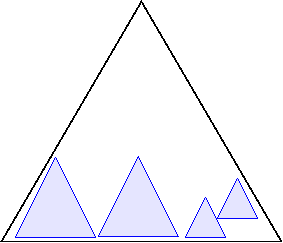
\includegraphics[width=2cm]{images/granularity1}\qquad
      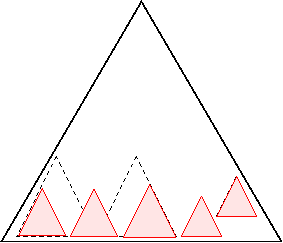
\includegraphics[width=2cm]{images/granularity2}
      \caption{Varying granularities.}
      \label{fig:granularity}
    \end{center}
  \end{minipage}
  \begin{minipage}{.33\linewidth}
  \begin{center}
    \leavevmode
    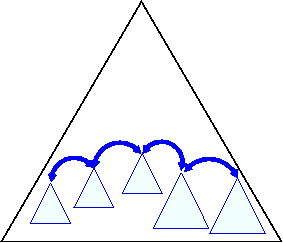
\includegraphics[width=2cm]{images/walker1}\qquad
    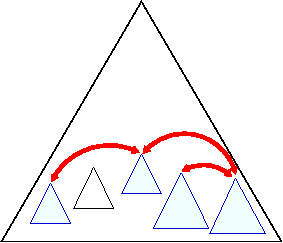
\includegraphics[width=2cm]{images/walker2}
    \caption{Different walkers.}
    \label{fig:walkers}
  \end{center}
\end{minipage}
  \begin{minipage}{.33\linewidth}
\begin{center}
    \leavevmode
    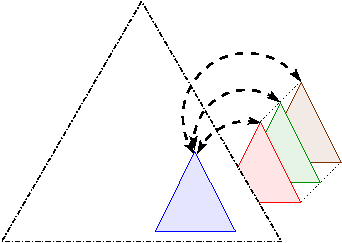
\includegraphics[width=2.5cm]{images/substructure1}
    \caption{Alternative representations.}
    \label{fig:alt}
  \end{center}
\end{minipage}
\end{figure*}

While granularities are generally structured from coarse grained to more fine
grained, this does not imply that they have to be strictly hierarchical. For
example, in text natural granularities are line, word or character. On the other
hand in more specialized content like a table one could distinguish
granularities like row, column, or cell, where the latter again can be segmented
by normal text granularities.  Defining granularities is therefore not
necessarily a simple task in particular due to often heavily nesting of layout
elements in rich web applications.

\subsection{Axis 2: Walking Content}
\label{sec:ax2}

Interactive navigation of content is accomplished by walkers.  They provide a
means to move between the different leaf nodes defined by a particular
granularity. They also offer the flexibility to break up the linear order of
navigating content as well as ignore certain leafs nodes. Fig.~\ref{fig:walkers} gives
an idea of different walkers operating on the same level of granularity.

The flexibility of the walkers is particular important to allow for a good user
experience on complex web content, where the ideal reading order is not
reflected by the order of the elements in the DOM. An example is the
\url{google.com} search page, which can contain in addition to the normal search
results additional information in the form of a knowledge card on the right or
timely information on the top (e.g., sports results). However, in the DOM the
knowledge card is given after all the search results, thus conventional linear
navigation would force the user to navigate through the entire list of search
results first before discovering the knowledge card.

In practice walkers and granularities are exposed to the user in meaningful
combinations only. Walkers usually group related granularities, whenever
possible in a hierarchical nature.  A user can not only switch explicitly
between levels of granularity but interactively walk at one level of
granularity, while if necessary exploring the currently active leaf node at the
next lower level of granularity.

For example, in default text walking mode granularities include line, word and
character. The user can either switch between these granularities, or while
walking the text linearly, for instance, in line granularity --- usually with up
and down arrow keys\footnote{These keys depend on the particular choice of
  keymap and possible user customization.}  --- explore the content of the line
that currently is being read, word for word using the left and right arrow keys.

Immediate keyboard shortcuts can be given to particular combinations of walker
and granularity. A particular example is the exploration of hyperlinks in a
document to which ChromeVox dedicates two keys explicitly for walking links
only, while ignoring all interspersed text.

\subsection{Axis 3: Speech Output}
\label{sec:ax3}

The third axis along which ChromeVox is customizable is how speech output is
generated. While the way regular text is read is determined by the TTS engine
employed and thus can not be influenced by ChromeVox directly, when conveying
additional information on content as well as while reading specialized content
flexibility on how elements are spoken or announced is important.

For example, ChromeVox can provide the user with context information on
particular elements, such as announcing the type of headers, whether a hyperlink
is contained etc., by announcing the element explicitly or playing
earcons. Simple adaptations of this behavior allows for changes
\begin{inparaenum}[(a)]
\item to the level of verbosity,
\item if and how punctuation is being read, and
\item to switch earcons on or off.
\end{inparaenum}

More complex structures can benefit from even more sophisticated customization.
For instance, when traversing tables ChromeVox can give the user information on
the current position in the table, for example, by announcing explicitly row and
column number or the cell type. Similarly, when speaking mathematics it can become
necessary to alter the pronunciation of elements or entire formulas according to
mathematical subject area or user preference.

For this purpose ChromeVox has a dedicated speech rule engine that allows to
specify speech rules for particular DOM elements. When a walker traverses a DOM
element for which a speech rule exists, it is used to generate speech
output. This can be a recursive process in the sense that the execution of one
speech rule might trigger further speech rules that apply to its sub-elements.
Customization is realized by defining different rules for elements and
parameterizing the engine swapping entire rule sets thus changing the generated
speech output.

As ChromeVox's speech rule engine has been designed originally in the context of
our work on mathematics and we shall present more details on
its operation and rule systems in Sec.~\ref{sec:translate}. However, the speech
rule engine has now been integrated as a general component into the screen
reader and can be employed to customize reading of any element in the DOM. In
fact, it is implemented in a general enough way that it allows to define and
recursively execute speech rules for any XML object, a fact that we can put to
use when working with alternative representations of DOM objects.


\subsection{Axis 4: Alternative Representations}
\label{sec:ax4}


The final axis of customization is ChromeVox's ability to swap entire elements
in the DOM for alternative representations. However, as we do not want to alter
the actual DOM, we achieve this by internally mapping particular leaf nodes to
dedicated representations. This idea is schematically depicted in
Fig.~\ref{fig:alt}.

% \begin{figure}[ht!]
%   \begin{center}
%     \leavevmode
%     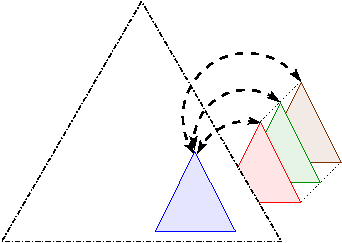
\includegraphics[width=.4\columnwidth]{images/substructure1}
%     \caption{Schematic depiction of alternative representations.}
%     \label{fig:alt}
%   \end{center}
% \end{figure}

We effectively allow any data structure as a valid alternative representation as
long as it is serializable into an XML representation. This allows us to define
bespoke speech rules for the resulting XML object and compile appropriate
speech output using the speech rule engine. Depending on the nature of the DOM
element to be replaced alternative representations are either pre-computed at
load time of a webpage or generated on the fly when the particular DOM object is
visited.

Employing alternative representations can be particularly beneficial when the
original DOM element is not suitable for speech generation or when a more
dedicated data structure can lead to a better understanding of the content
for the user. Its use can either be triggered automatically, or explicitly by a
user command. In fact, this ability plays a crucial role in the accessibility of
mathematical content and we describe it in more detail in
Sec.~\ref{sec:alternative}.


\section{Speaking Mathematics}
\label{sec:translate}

The speech translation of mathematics poses some unique difficulties which makes
it a more challenging task for a screen reader than the aural
rendering of text. When for regular text it is generally enough to identify what
needs to be spoken possibly together with the language it is in, and let a TTS
engines take care of deciding how the text is voiced by adding appropriate
prosody etc., for mathematical expressions much of the heavy lifting has to be
done by the screen reader by translating formulas into an utterance the ensures
the TTS, which is normally geared towards speaking continuous text, voices them
appropriately for the following reasons:

\begin{itemize}\itemsep-1pt
\item Mathematical notation uses a much wider spectrum of symbols than ordinary
  text, most of which have to be translated by the screen reader into a
  meaningful expression before sending it to the TTS.
\item Punctuation is often crucial for the understanding of a formula. Thus
  symbols like periods, commas, and parentheses either have to be pronounced
  explicitly or modeled by appropriate pausing. 
\item Even white space that would normally be ignored can have meaning in a
  formula (e.g., elided operation symbols, function applications) and needs
  to be pronounced.
\item Formulas often exhibit a two dimensional layout that has to be conveyed to
  a reader, either by changes in intonation or by making explicit announcements.
  Furthermore, formulas can be nested arbitrarily deep, adding the need to
  communicate that complexity.
\item There is no standardized mathematical language or dictionary that allows
  us to retrieve the proper pronunciation of symbols or expressions. Moreover,
  meaning can vary across different mathematical domains.
\end{itemize}

We tackle these challenges by providing a simple, yet powerful enough rule
language to translate both single symbols and complex expressions, that
furthermore can be specialized with respect to mathematical domains and user
preferences.

\subsection{Describing Math via Speech Rules}

\newcommand{\srule}[2]{\ensuremath{#1 \rightarrow #2}}
\newcommand{\slist}[1]{\ensuremath{#1}}
\newcommand{\ttrule}[2]{
  
  \noindent\centerline{\texttt{#1}$\rightarrow$\texttt{#2}}}
\newcommand{\tttrule}[2]{

  \noindent
  \texttt{#1}\newline\hspace*{\fill}$\longrightarrow$\texttt{#2}

}
\def\cR{{\cal R}} \def\cN{{\cal N}} \def\assign#1#2{{#1}\leftarrow{#2}} 


The primary means to translate mathematical expressions is the speech rule
engine described in Sec.~\ref{sec:ax3}. In fact the engine and its rule language
was originally designed in the context of speaking mathematical expressions.

The basic structure of a rule is that of a \emph{condition/action pair}, where
the condition decides on the applicability of a rule to a DOM element and the
action contains instructions how to construct speech output for the element
that can be passed to a TTS. More formally we define a rule as:
\[R= ({C},{A}) = \srule{\slist{c_0;\ldots;c_n}}{\slist{a_0;\ldots;a_m}} \] where
$C$ is a non-empty ordered list of \emph{Xpath expressions}~\cite{clark1999xpl} and
$A$ is a non-empty ordered list of \emph{action components}.

In detail, the condition $C=\slist{c_0;\ldots;c_n}$ consists of a mandatory
element $c_0$, which is an Xpath node selector, and a set of optional $c_i,
i=1,\ldots,n$, which are Xpath predicates. The rule $R$ is applicable to a DOM
node $N$, if $c_0$ returns $N$ and all other $c_i$ hold for $N$.

The speech output for $N$ is then computed using the action $A =
\slist{a_0;\ldots;a_m}$, where each action component $a_i, i=0,\ldots,n$
consists itself of three parts: 
\begin{description}\itemsep-1.5pt
\item[Type] specifies how the component is treated by the speech rule engine. We
  distinguish four types of components:
  \begin{description}\itemsep-1.5pt
  \item[Node (denoted \texttt{n})] A single node that is recursively given to
    the rule engine.
  \item[Multi (\texttt{m})] A list of nodes is passed to the engine.
  \item[Text (\texttt{t})] Content that is given directly to the TTS.
  \item[Personality (\texttt{p})] Customizes the behavior of the TTS.
  \end{description}
\item[Content] is, depending on the type of the component, either an Xpath
  expression returning a node or a list of nodes, for types \texttt{n} and
  \texttt{m}, respectively, or a string or an Xpath expression returning a
  string for type \texttt{t}.  It is empty for type \texttt{p}.
\item[Annotation] specifies additional parameters that influence the execution
  of the component or the TTS behavior.
\end{description}

As examples of a simple rule consider the following the rule for an \texttt{mi}
element: \ttrule{self::mathml:mi}{[t] text()} Here the condition simply states
that the node itself has to have the tag \texttt{mi}. As MathML has its own name
space in HTML, we have to include it as prefix in the Xpath expression. The
action of the rule has a single component of text type, which simply returns the
content of the node. Observe that we write types in square brackets, while
writing annotations in round parentheses following the Xpath
expression. Annotations can be omitted.

Given our definition of rules we can now describe the basic working of the
speech rule engine in pseudo-code. The engine is parameterized with a set of
speech rules ${\cR}={\{R_1,\ldots,R_n\}}$ and applied to a DOM node $\cN$.

\vspace{.3cm}\hrule\vspace{.2cm}
\noindent \textbf{SpeechRuleEngine}($\cR$, $\cN$)
\vspace{-.2cm}\begin{ntabbing}
  mi\=mi\=mi\=mi\=mi\=mi\=mi\=mi\=\kill
  let applicable rules $\assign{S}{\emptyset}$\label{}\\
  for each $R\in \cR$\label{}\\
  \> assume $R$ is of the form $\srule{\slist{c_0;\ldots;c_n}}{A}$\label{}\\
  \> if $c_0(N) = N$ and $c_i(N) = \mathbf{true}, i=1,\ldots,n$\label{}\\
  \>\> $\assign{S}{S\cup\{R\}}$\label{}\\
  if $S=\emptyset$\label{}\\
  \> speak text content of $\cN$\label{line:default}\\
  else \label{}\\
  \> $\assign{R}{\mbox{pick from }S}$ \label{line:heuristic}\\
  \> assume $R$ is of the form $\srule{C}{a_0;\ldots;a_m}$\label{}\\
  \> for each $a_i, i=0,\ldots,m$\label{}\\
  \>\>case type of $a_i$ is\label{}\\
  \>\>\>n:\> $\assign{\cN'}{\mbox{apply content of } a_i}$\label{line:case-n}\\
  \>\>\>\>\textbf{SpeechRuleEngine($\cR$, $\cN'$)}\label{}\\
  \>\>\>m:\> $\assign{\cN_1',\ldots,\cN_k'}{\mbox{apply content of } a_i}$\label{line:case-m}\\
  \>\>\>\>for each $\cN_i', i=1,\ldots,k$\label{}\\
  \>\>\>\>\>\textbf{SpeechRuleEngine($\cR$, $\cN_i'$)}\label{}\\
  \>\>\>t:\>speak content of $a_i$\label{line:case-t}\\
  \>\>\>p:\>execute annotation of $a_i$\label{line:case-p}\\
\end{ntabbing}
\vspace{-.5cm}\hrule\vspace{.2cm} 

Note, that in line~\ref{line:heuristic} we have not fully specified how a rule $R$ is
picked from the set of all applicable rules. Here we can apply a heuristic on
rule preference, which currently defaults to the most constraint rule in the
set.

Note also, that we can not guarantee termination of our procedure, as our rules
allow for arbitrary Xpath expressions, which can move along all axes in the DOM,
hence we could easily construct a set of cyclic rules. On the other hand we can
have incomplete rule sets as in case no further rule is applicable,
line~\ref{line:default} specifies that the text content of the current node is
spoken, which is computable for any node in the DOM. Indeed this is a potential
way to deal with text nodes. However, we can also deal text content explicitly
which we indeed do for the majority of Unicode characters.  The following is a
rule dealing with the plus minus symbol in the quadratic formula:
\ttrule{self::text(); ./text()=\&\#x00B1}{[t] "plus minus"} The rule has two
conditions: The first returns the node if it is a text node, while the second
tests for the Unicode character. If the rule is applicable its sole action as
per line~\ref{line:case-t} of our procedure is to speak the content
``plus minus''.

To illustrate the other cases we first consider the following rule that is
applicable if we have a \texttt{msup} node whose second child, i.e., the superscript is
equal to $2$: \tttrule{self::mathml:msup; ./*[2][text()=2]}{[n] ./*[1]; [t]
  "square"} The rule's action specifies first that first the content of the
first child node is spoken by applying the engine's procedure recursively
(line~\ref{line:case-n}), followed by speaking the string ``square''.  We can
observe that the rule is indeed applicable to the \texttt{msup} node in
Fig.~\ref{fig:quadratic-mml}.

For the remaining cases  consider the square root rule:
\tttrule{self::mathml:msqrt}{[t] "Square root of"; [m] ./*; [p] (pause:400)}

\noindent When its action is executed, it
\begin{inparaenum}[(1)]
\item first sends the string ``Square root of'' to the TTS.
\item Then the multi type component retrieves the list of all child nodes of the
  \texttt{msqrt} node and applies the speech rule engine to each of the children.
\item Finally the last component is of personality type, implying that it
  has no content but only send instructions to the TTS, which in this case is a
  pause of 400ms.
\end{inparaenum}

For simplicity we have not given any details how annotations are executed.
Moreover, we have also omitted the details that additional annotations might
need to be executed in the case of type $n$, $m$, and $t$. We rather explain
this at the hand of a concrete example. Consider the following speech rule for
\texttt{mfenced} elements:

\noindent\texttt{self::mathml:mfenced;}\\
\hspace*{.5cm}\texttt{string-length(string(@separators))=1} $\longrightarrow$ \\
\hspace*{\fill}\texttt{[t] @open; [m] ./* (separator:@separators);}\\
\hspace*{\fill}\texttt{[t] @close} 

\noindent The rule is applicable to
any \texttt{mfenced} node that has \texttt{separators} attribute that contains exactly one
character. Its action has the notable features that
\begin{inparaenum}[(a)]
\item the first and last utterance are constructed by Xpath expressions
  accessing the node's attributes \texttt{open} and \texttt{close},
  respectively. And
\item that the multi component has a separator annotation, which specifies that a
  string that is spoken between every element in the list of child nodes. In our
  case this is the content of the \texttt{separators} attribute again retrieved with an
  Xpath expression.
\end{inparaenum}
For example applying the rule to the MathML markup 

{\lstxml\small
\begin{lstlisting}
<math xmlns="http://www.w3.org/1998/Math/MathML">
  <mfenced open="{" close="}" separators=";">
    <mi>a</mi><mi>b</mi><mi>c</mi>
  </mfenced></math>
\end{lstlisting}}
\noindent will result in speech output for the expression $\{a;b;c\}$.

Similar to the separator annotation we allow for a \texttt{context} annotation,
which is spoken for every element.  In addition we also offer attributes to
change the behavior of the TTS, similar to pause, which play a major role in
the next section.

% Observe that we can define rules for any node in the tree by testing its
% applicability with an Xpath expression. This does not only mean that the rules
% are not restricted to MathML markup, but also that we can specify translation
% rules for single characters or strings. 


% \tttrule{self::span[\@class="mfrac"]}{[n] ./*[1]/*[1]/*[1]; [t] "divided by"; [n] ./*[1]/*[2]/*[1]}

% and a MathJax rule for fractions



\subsection{Conveying Meaning by Intonation}

As mathematical expressions can be arbitrarily complex and deeply nested
conveying their extend and two dimensional layout in speech is very challenging.
A traditional approach to explain two dimensional structures as well as nesting
depth is to insert additional vocabulary that gives the relative position of
expressions, which can make spoken expressions very cumbersome and long.
Another approach, originally presented in~\cite{raman1994aster}, is to take
advantage of the precision a TTS engine offers to control exactly variations in
intonation, which goes beyond what a human could do.

In ChromeVox we allow for both models. The former is easy to achieve by adding
appropriate vocabulary to the rules. The latter can be done by specifying
intonation changes as annotations of our speech rule actions. An intonation
change given in an action of type $t$ or $p$ will only affect a single
utterance, while for types $n$ and $m$ the changes are applied recursively,
and multiple recursive changes to a particular intonation parameter are summed
up, thus enabling to convey nesting depth and two dimensional structure of an
expression.  In particular, we allow for the variation of
\begin{inparaenum}[(1)]
\item speech pitch,
\item speech rate,
\item volume, as well as the inclusion of
\item pauses and
\item earcons.
\end{inparaenum}

As example consider the following fraction rule:

\noindent\texttt{self::mathml::mfrac}$\longrightarrow$
\texttt{[n] ./*[1] (pitch:0.3);}\newline
\hspace*{\fill}\texttt{[t] "over"; [n] ./*[2] (pitch:-0.3)}

\noindent 
Spatial layout is conveyed by raising the pitch when moving up and lowering it
when moving down. These are the effects on some simple, yet challenging
expressions taken from~\cite{knuthart}.
\tabcolsep1pt
\begin{tabular}{lp{.7\textwidth}}
  $x+y^2\over k+1$ &
  $\framebox{\text{x plus y square}}_{.3}$ 
  $\framebox{\text{over}}_{0}$ 
  $\framebox{\text{k plus one}}_{-.3}$
  \\
  ${x+y^2\over k}+1$ &
  $\framebox{\text{x plus y square}}_{.3}$
  $\framebox{\text{over}}_{0}$
  $\framebox{\text{k}}_{-.3}$
  $\framebox{\text{plus one}}_{0}$
  \\
  $x+{y^2\over k+1}$ &
  $\framebox{\text{x plus}}_{0}$
  $\framebox{\text{y square}}_{.3}$
  $\framebox{\text{over}}_{0}$
  $\framebox{\text{k plus one}}_{-.3}$
  \\
  $x+{y^2\over k}+1$ &
  $\framebox{\text{x plus}}_{0}$
  $\framebox{\text{y square}}_{.3}$
  $\framebox{\text{over}}_{0}$
  $\framebox{\text{k}}_{-.3}$
  $\framebox{\text{plus one}}_{0}$
  \\
% $x+y^{2\over k+1}$ & x plus y square over k plus one\\
\end{tabular}
Working in addition with rate and pauses, e.g., before and after a fraction, in
the rules can make for a concise but nevertheless ambiguity free reading
experience.

% \[ {x^2}^y = x^{2y}\]

%\enlargethispage{.2cm}
\subsection{Customizing Rule Sets}

Since mathematical symbols and expressions can have quite different meaning in
different mathematical subject areas despite being represented similarly, it is
important to allow for customization of rule sets. Rules in ChromeVox can be
defined with respect to a mathematical domain (e.g., algebra, geometry,
calculus) and a reading style (e.g., verbose, brief). This is additional
administrative information specified when a rule is defined, which we omit here
to preserve space.

ChromeVox contains default rule sets for MathML and MathJax expressions as well
as for semantic interpretations discussed in Sec.~\ref{sec:semantic}. They are
used in case no more specialized rules are available for a mathematical domain
or reading style.  Customization can be done either by the content provider or
by the user. For the former case ChromeVox offers an API that allows a web site
author to include specialist reading rules that can be picked up by ChromeVox
when a user is visiting the page.

Suppose we want to read the following logical inference rule correctly,
that is given in MathML on the right:

\begin{minipage}{.4\linewidth}
  \[\frac{\varphi}{\neg\neg \varphi}\]
\end{minipage}
\begin{minipage}{.55\linewidth} {\lstxml\small
\begin{lstlisting}
<mfrac><mrow>
    <mo>&#x00AC;</mo>
    <mo>&#x00AC;</mo>
    <mi>&#x03C6;</mi>
  </mrow>
  <mi>&#x03C6;</mi></mfrac>
\end{lstlisting}
  }
\end{minipage}
We can add the following rule for the logic domain:
\tttrule{self::mathml::mfrac}{[n] ./*[2]; [t] "follows from"; [n] ./*[1]} 
\noindent Thus when the logic domain is selected the above expression would be
pronounced ``Not not phi follows from phi'' instead of as a fraction as by
default.

In practice the user can cycle through both mathematical domains and reading
styles to parameterize the speech rule engine. The engine is invoked whenever a
MathML (or MathJax) expression or sub-expression is encountered. When in
continuous reading mode math expressions are always spoken in their
entirety. When interacting with content in some text granularity (with the
notable exception of the character granularity), math expressions are
effectively considered as leafs, regardless of the actual granularity.

In both cases the math expression is explicitly pointed out to the user by
ChromeVox playing an earcon and, if in verbose mode, also announcing
``Math''. This is a means to alert the user not only to the existence of math in
the text but also to the possibility that they can further engage with the
expression by exploring it interactively.

\enlargethispage{.5cm}
\section{Engaging with Formulas}
\label{sec:explore}

\begin{figure*}[t!]
  \centering
  \tabcolsep1pt{\footnotesize
    \noindent\begin{tabular}{clclclclclcl}
      & $\framebox{$x=\frac{-b \pm \sqrt {b^2-4ac}}{2a}$}$  & $\longleftrightarrow$ 
      & $\framebox{$x$}=\frac{-b \pm \sqrt {b^2-4ac}}{2a}$  & $\longleftrightarrow$ 
      & $x\framebox{$=$}\frac{-b \pm \sqrt {b^2-4ac}}{2a}$  & $\longleftrightarrow$ 
      & $x=\framebox{$\frac{-b \pm \sqrt {b^2-4ac}}{2a}$}$  & $\longleftrightarrow$ 
      & $x=\frac{\framebox{$-b \pm \sqrt {b^2-4ac}$}}{2a}$\\
      $\longleftrightarrow$ 
      & $x=\frac{\framebox{$-$}b \pm \sqrt {b^2-4ac}}{2a}$  & $\longleftrightarrow$ 
      & $x=\frac{-\framebox{$b$} \pm \sqrt {b^2-4ac}}{2a}$  & $\longleftrightarrow$ 
      & $x=\frac{-b\framebox{$\pm$} \sqrt {b^2-4ac}}{2a}$  & $\longleftrightarrow$ 
      & $x=\frac{-b\pm\framebox{$\sqrt {b^2-4ac}$}}{2a}$  & $\longleftrightarrow$ 
      & $x=\frac{-b\pm\sqrt {\framebox{$b^2$}-4ac}}{2a}$\\
      $\longleftrightarrow$ 
      & $x=\frac{-b\pm\sqrt {\framebox{$b$}^2-4ac}}{2a}$  & $\longleftrightarrow$ 
      & $x=\frac{-b\pm\sqrt {b^{\framebox{$2$}}-4ac}}{2a}$  & $\longleftrightarrow$ 
      & $x=\frac{-b\pm\sqrt {b^2\framebox{$-$}4ac}}{2a}$  & $\longleftrightarrow$ 
      & $x=\frac{-b\pm\sqrt {b^2-\framebox{$4$}ac}}{2a}$  & $\longleftrightarrow$ 
      & $x=\frac{-b\pm\sqrt {b^2-4\framebox{$a$}c}}{2a}$\\
      $\longleftrightarrow$ 
      & $x=\frac{-b\pm\sqrt {b^2-4a\framebox{$c$}}}{2a}$  & $\longleftrightarrow$ 
      & $x=\frac{-b\pm\sqrt {b^2-4ac}}{\framebox{$2$}a}$  & $\longleftrightarrow$ 
      & $x=\frac{-b\pm\sqrt {b^2-4ac}}{2\framebox{$a$}}$
    \end{tabular}}
  \caption{Tree exploration of the quadratic formula.}
\label{fig:tree-exploration}
\end{figure*}


Mathematical formulas are generally of a complex nature, in fact, already a
small number of symbols can make for a complex utterance.  Consequently, just
listening to an expression once is generally not enough for a user to fully take
in its meaning.  Therefore for mathematical formulas it is particularly
important to be able to engage with them interactively by offering means of
traversing sub-expressions.  ChromeVox offers these facilities with its concepts
of granularities and walkers. However, as opposed to many other form of content,
such as regular text, mathematical formulas can be nested arbitrarily deep,
meaning that an expression can have sub-expressions of the same or higher
complexity. Consequently, the standard approach of having a standard set of
roughly ordered granularities that enable a user to descend into an expression
can not work for mathematical formulas. Instead we need specialist walkers and a
concept of nested granularity to allow for meaningful exploration. Therefore, we
have experimented with two different approaches walking MathML expressions:
\begin{enumerate}[(1)]
\item \emph{Tree exploration} follows closely the tree structure of a MathML expression.
\item \emph{Level based exploration} defines a granularity of
  sub-ex\-pressions and allows to dive into each of these separately.
\end{enumerate}
We now render those notions more precisely.

Let $T=(V,E)$ be a rooted tree with root $r\in V$ in the usual graph theoretic
sense (i.e., a directed acyclic graph, with all edges directed away from the
root and all child nodes having only one parent).  Let $V=\{v_0=r,\ldots,v_n\}$
given in a pre-ordering. We then define a granularity $G=\{t_0,\ldots, t_n\}$,
where $t_i$ is a sub-tree of $T$ with root $v_i$, $i=0,\ldots,n$. Note that
$t_0=T$. We then define \emph{tree exploration} on $T$ as linearly walking on
the elements of $G$, that is, walking forward corresponds to shifting from $t_i$
to $t_{i+1}$, $i=0,\ldots,n-1$ and likewise walking backwards to moving from
$t_i$ to $t_{i-1}$, $i=1,\ldots, n$.

This effectively means that the granularity consists of every sub-tree of the
expression or in other words tree exploration corresponds to depth first
traversal of the sub-trees in $T$. Since we are exploring trees that are
elements of the DOM, the order of the vertices is naturally given by the
ordering of the nodes in the DOM.


\begin{figure*}[ht!]
  \centering
\tabcolsep2pt\small
\noindent\begin{tabular}{lclclclcll}
  \multicolumn{1}{c}{Level 0} &  & \multicolumn{1}{c}{Level 1} & & 
  \multicolumn{1}{c}{Level 2} & & \multicolumn{1}{c}{Level 3} & & 
  \multicolumn{1}{c}{Level 4}\\
$\framebox{$x=\frac{-b \pm \sqrt {b^2-4ac}}{2a}$}$  & $\longleftrightarrow$ 
& $\framebox{$x$}=\frac{-b \pm \sqrt {b^2-4ac}}{2a}$  &  \\
& & $x\framebox{$=$}\frac{-b \pm \sqrt {b^2-4ac}}{2a}$  &  \\
& & $x=\framebox{$\frac{-b \pm \sqrt {b^2-4ac}}{2a}$}$  & $\longleftrightarrow$ 
& $x=\frac{\framebox{$-b \pm \sqrt {b^2-4ac}$}}{2a}$  & $\longleftrightarrow$ 
& $x=\frac{\framebox{$-$}b \pm \sqrt {b^2-4ac}}{2a}$  \\
& & & & & & $x=\frac{-\framebox{$b$} \pm \sqrt {b^2-4ac}}{2a}$ \\
& & & & & & $x=\frac{-b\framebox{$\pm$} \sqrt {b^2-4ac}}{2a}$ \\
& & & & & & $x=\frac{-b\pm\framebox{$\sqrt {b^2-4ac}$} }{2a}$ & $\longleftrightarrow$ 
& $x=\frac{-b\pm\sqrt {\framebox{$b^2$}-4ac} }{2a}$ & $\longleftrightarrow\cdots$\\
& & & & & & & & $x=\frac{-b\pm\sqrt {b^2\framebox{$-$}4ac} }{2a}$\\[.2cm]\cline{7-7}
& & & & $x=\frac{-b \pm \sqrt {b^2-4ac}}{\framebox{$2a$}}$  & $\longleftrightarrow$ 
& $x=\frac{-b \pm \sqrt {b^2-4ac}}{\framebox{$2$}a}$ & & \multicolumn{1}{c}{\vdots}\\
& & & & & & $x=\frac{-b \pm \sqrt {b^2-4ac}}{2\framebox{$a$}}$ 
\end{tabular}
  \caption{Level exploration of the quadratic formula.}
\label{fig:level-exploration}
\end{figure*}

If we consider again our example of the quadratic formula, then the MathML tree
has the following form, where the topmost \texttt{math} tag is the root:

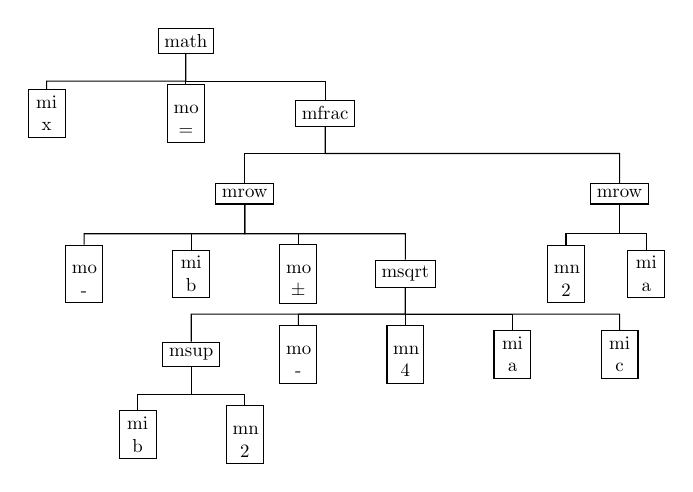
\begin{tikzpicture}[scale=.68, transform shape]
\node[draw] {math}
  %%[edge from parent fork down]
  [grow via three points={one child at (0,-1.25) and two children at (-1.3,-1.3) and (1.3,-1.3)}, edge from parent fork down]
    child {node[draw]{\begin{minipage}{3ex}\begin{center}mi\\\textcolor{black}{x}\end{center}\end{minipage}}}
    child {node[draw]{\begin{minipage}{3ex}\begin{center}mo\\\textcolor{black}{=}\end{center}\end{minipage}}}
    child {node[draw] {mfrac}[grow via three points={one child at (0,-1.5) and two children at (-1.5,-1.5) and (5.5,-1.5)}, edge from parent fork down]
      child {node[draw] {mrow}[grow via three points={one child at (0,-1.5) and two children at (-1,-1.5) and (1,-1.5)}, edge from parent fork down]
        child {node[draw]{\begin{minipage}{3ex}\begin{center}mo\\\textcolor{black}{-}\end{center}\end{minipage}}}
        child {node[draw]{\begin{minipage}{3ex}\begin{center}mi\\\textcolor{black}{b}\end{center}\end{minipage}}}
        child {node[draw]{\begin{minipage}{3ex}\begin{center}mo\\\textcolor{black}{$\pm$}\end{center}\end{minipage}}}
        child {node[draw] {msqrt}[grow via three points={one child at (0,-1.5) and two children at (-1,-1.5) and (1,-1.5)}, edge from parent fork down]
          child {node[draw] {msup}[grow via three points={one child at (0,-1.5) and two children at (-1,-1.5) and (1,-1.5)}, edge from parent fork down]
            child {node[draw]{\begin{minipage}{3ex}\begin{center}mi\\\textcolor{black}{b}\end{center}\end{minipage}}}
            child {node[draw]{\begin{minipage}{3ex}\begin{center}mn\\\textcolor{black}{2}\end{center}\end{minipage}}}
          }
          child {node[draw]{\begin{minipage}{3ex}\begin{center}mo\\\textcolor{black}{-}\end{center}\end{minipage}}}
          child {node[draw]{\begin{minipage}{3ex}\begin{center}mn\\\textcolor{black}{4}\end{center}\end{minipage}}}
          child {node[draw]{\begin{minipage}{3ex}\begin{center}mi\\\textcolor{black}{a}\end{center}\end{minipage}}}
          child {node[draw]{\begin{minipage}{3ex}\begin{center}mi\\\textcolor{black}{c}\end{center}\end{minipage}}}
        }
      }
      child {node[draw] {mrow}[grow via three points={one child at (0,-1.5) and two children at (-1,-1.5) and (.5,-1.5)}, edge from parent fork down]
        child {node[draw]{\begin{minipage}{3ex}\begin{center}mn\\\textcolor{black}{2}\end{center}\end{minipage}}}
        child {node[draw]{\begin{minipage}{3ex}\begin{center}mi\\\textcolor{black}{a}\end{center}\end{minipage}}}
      }
    }
    ;
\end{tikzpicture}

The single steps of the tree exploration of the above tree are given in
Fig.~\ref{fig:tree-exploration}.  The framed sub-expressions correspond to the
sub-formulas that are being spoken in each step.  Notice that tree exploration
allows us to walk continuously from the root of the tree to the rightmost leaf
node, without the need to explicitly change granularity.

Experimenting with tree exploration showed, that while it gave a pretty good
idea of the overall layout of a formula, it was not well suited to convey the
internal sub-structuring of many expressions. Consequently, we designed a second
exploration method that aims to offer tighter control on the exploration of
sub-expressions.

As for tree exploration we let $V=\{v_0=r,\ldots,v_n\}$ given in a pre-ordering
and the set of sub-trees in $T$ as $S=\{t_0,\ldots, t_n\}$ equivalent to the $G$
in the previous definition. In addition, we define usual \emph{depth of a node}
in $V$, that is, $v_i$ is at depth $d$ if the path from $v_0$ to $v_i$ has $d$
edges. We now recursively define the granularities by level:
\begin{enumerate}[(i)]
\item Let $G_0=\{t_0\}$ be the granularity at level $0$.
\item Let $t\in G_\ell$. We define the granularity at level $\ell + 1$ as
  \arraycolsep1pt
  \begin{eqnarray*}
    G^t_{\ell+1} = \{s\in G & | & s \mbox{ is sub-tree of } t\mbox{ and }\\ 
    & & \mbox{root of } s \mbox{ is at depth } \ell+1\}.
  \end{eqnarray*}
\end{enumerate}
Observe that this definition means that granularities are defined relative to
sub-expressions, that is, the granularity $G^t_{\ell+1}$ are only the proper
sub-trees of the level $\ell$ node. Consequently, there exists a level $\ell+1$
granularity for every vertex at depth $\ell$ that is not a leaf
node. Furthermore, when walking a $\ell+1$ level granularity, we can not leave
the common expression defined by the common parent node.

The level exploration for equation~(\ref{eq:quadratic}) is partially
displayed in~\ref{fig:level-exploration}, where framed sub-expressions correspond
again to the sub-formulas that are spoken. Columns correspond to the different
levels of granularities and arrows between levels indicate that the framed
sub-expression can be explored at the next lower level. Exploration of
expressions at the same granularity corresponds to moving up and down in a
column. However, observe that the horizontal bar in level $3$ indicates the
boundary between two level $2$ granularities, where the entries above the bar
belong to $G^{-b\pm\sqrt{b^2-4ac}}_2$ and the ones below to $G^{2a}_2$. Hence one
can not move from the enumerator to the denominator and if we wanted to explore
the sub-expressions in the denominator (i.e., $2$ and $a$), we have to first move
back up to the second level, move to the expression $2a$ and can then explore
the next lower level.

Level exploration fits naturally into ChromeVox's paradigm of engaging with
content at different levels of granularities. As with regular text content the
user can explore an expression in two ways. They can move between expressions at
one level with up and down arrow keys, while exploring the currently active
sub-expression at the next lower level with the left and right arrow
keys. Furthermore, the usual key combinations to change granularities allow the
user to move up and down the different levels. These are announced explicitly to
give the reader a feel for the depth of an expression.  When a user tries to go
beyond the boundaries of an expression during exploration an earcon is
played. Similarly the earcon announces when the user tries to descend further
beyond the lowest level of a sub-expression.

Interactive exploration is available for both math expressions given in MathML
syntax and rendered with MathJax. While in the case of the former we walk along
the tree structure defined precisely by the MathML tags, in the case of the
latter we walk the tree structure given by \texttt{span} nodes whose additional
class attribute mirrors the MathML tag. This has the advantage that in addition
to aurally render sub-expressions, we can also make use of ChromeVox's visual
indicator --- a tool that allows users with low vision or reading disorders to
follow the flow of the text --- to highlight the sub-expressions currently being
explored. Beyond exploring elements inside the DOM interactive exploration is
also possible for alternative representations that ChromeVox can use for math
expressions and that are presented in the following section.

\section{Re-representing Math Content}
\label{sec:alternative}

ChromeVox's ability to allow for alternative representations as discussed in
Sec.~\ref{sec:ax4} is crucial for both enlarging the amount mathematical content
available and the user experience when voicing that content. In fact, we have
developed the mechanism initially in the context of math accessibility for two
purposes:
\begin{enumerate}
\item As much of mathematics on the web is still only available as
  pre-rendered images as described in Sec.~\ref{sec:images}, we exploit any
  alternative markup we can find to internally replace the image representation
  thus making the expression accessible.
\item Since the direct translation of MathML expressions leads to speech output
  that is rather verbose and often differs quite significantly how a human
  reader would speak a formula, we have developed a more semantic interpretation
  of expressions as alternative.
\end{enumerate}

\subsection{Replacing Images}
\label{sec:images}

One major advancement for the accessibility of mathematics on the web is to make
hidden markup available to a screen reader, as much of the formulas on some of
the major sites providing mathematical content are still given in image format.
In ChromeVox we achieve this by explicitly looking for images of a particular
class.  For example, in Wikipedia \texttt{img} tags with the \texttt{class}
attribute \emph{tex} indicate that there is a math expression given as rendered
image with its {\LaTeX} source in the \texttt{alt} attribute.  Similarly, in
MathWorld a number of different \texttt{class} attributes in \texttt{img} tags
indicate that there is AsciiMath in the \texttt{alt} attribute that can be
exploited.

Unfortunately, using markup like {\LaTeX} or AsciiMath directly in ChromeVox is
not easily feasible as ChromeVox is built to use the HTML DOM to generate speech
output. Moreover, adding another two markup languages, would not only multiply
the number of rules necessary for their speech translation thus increasing
maintenance effort, but also make it very difficult to achieve consistency
between aural rendering of the same formula given in different formats.

We have therefore decided to translate all hidden markup into MathML allowing us
to utilize all the facilities we have built for it already. In order not to
duplicate efforts by writing our own translation engine as well as to ensure
further consistency between translated hidden markup and the same markup
rendered visually with MathJax, we are using MathJax for the translation of
hidden markup by employing it effectively as a web service.

Technically this is realized by implementing a bridge to MathJax from within the
the web page. We inject a MathJax configuration script into the web page's
content to allow ChromeVox to call MathJax remotely. For each of the math images
we have identified we send the hidden markup (i.e., either {\LaTeX} or
AsciiMath) to MathJax to obtain a corresponding MathML representation. The
MathML is computed upon loading of a web page and stored to be available as soon
as the screen reader encounters an image with a math formula. If stored MathML
markup exists, it is automatically retrieved and send to the speech rule engine
to generate the audio description. Note that this will not change the actual
image node in the DOM.

For example, when loading the Wikipedia page on the quadratic formula, ChromeVox
will detect the markup given in Fig.~\ref{fig:quadratic-img}, find the hidden
{\LaTeX} markup and send it to MathJax for translation, resulting in the MathML
expression given in Fig.~\ref{fig:quadratic-mml}. The latter is then actually
passed to the speech rule engine whenever the screen reader encounters the
original \texttt{img} node.

In addition to translating the MathML markup for the entire expression,
ChromeVox also enables the interactive exploration of the expression as
described in Sec.~\ref{sec:explore}, as if the node were an element of the
DOM. The only difference is that the visual indicator that highlights
sub-expression, when they are traversed, can not do the same as only the image is
contained in the web page.


\subsection{Semantic Representations}
\label{sec:semantic}

So far we have exclusively worked with MathML (or MathJax) representation of
expressions to generate speech output. But although a tree representation,
presentation MathML is optimized towards the visual rendering rather than
correct mathematical interpretation.  Consequently, the speech output is very
verbose, in that every single symbol in an expression is pronounced, while still
quite removed from what a human would say. If math is read by a human
expert they instantly interpret symbols and expressions in context of the
overall formula and adjust their speech accordingly by, for example, omitting
certain punctuation while selecting to pronounce other, elided notation.

For example, when reading $g(a+b)=g(a) + g(b)$ an expert reader would normally
interpret $g$ as a function and say ``g of a plus b'' as they can look beyond the
equality sign and put $g$ in context. Given a flat MathML structure this is
effectively not possible, or at least not without writing very elaborate, but
potentially fragile, speech rules.

We have decided to forgo this and rather exploit the possibility of using
alternative representations and to rewrite math expressions into a dedicated
semantic representation.  The idea is to interpret MathML in a semantic that
is modeled at K-12 and undergraduate mathematics.

In detail the procedure follows a heuristic approach that aims to represent a
formula in a semantic tree structure that is more akin to a term tree. The
semantic tree is assembled bottom-up, that is we first classify the single
components of an expression, giving each an immutable type and a mutable
role. The former aims to capture the basic nature of the symbol, while the
latter is used to describe the role of a symbol in the context of the formula.
For example, $f$ which has the type Latin letter can have the role of an
identifier in $f + g$ while that of a function in $f(x)$.

A central heuristic then builds term trees from flat structures by promoting
relations and defining operator precedence orders as well as determining
properly delimited structures. As an example of this heuristic we observe how the quadratic
formula is rewritten to its semantic interpretation below:

\begin{tikzpicture}[scale=.68, transform shape]
  \node[draw] {=}
  [grow via three points={one child at (0,-1.25) and two children at (-2.3,-1.3) and (2.3,-1.3)}, edge from parent fork down]
  child {node[draw] {x}}  
  child {node[draw] {/}[grow via three points={one child at (0,-1.3) and two children at (-1.3,-1.3) and (5.5,-1.3)}, edge from parent fork down]
    child {node[draw] {$\pm$}[grow via three points={one child at (0,-1.3) and two children at (-1,-1.3) and (3,-1.3)}, edge from parent fork down]
      child {node[draw] {-}[grow via three points={one child at (0,-1) and two children at (-1,-1.3) and (1,-1.3)}, edge from parent fork down]
        child {node[draw]{b}}}
      child {node[draw] {sqrt}[grow via three points={one child at (0,-1) and two children at (-1,-1.3) and (1,-1.3)}, edge from parent fork down]
        child {node[draw] {-}[grow via three points={one child at (0,-1) and two children at (-2,-1.3) and (2,-1.3)}, edge from parent fork down]
          child {node[draw] {$\,\widehat{}\,$}[grow via three points={one child at (0,-1.3) and two children at (-1,-1.3) and (1,-1.3)}, edge from parent fork down]
            child {node[draw]{b}}
            child {node[draw]{2}}}
          child {node[draw] {$\cdot$}[grow via three points={one child at (0,-1.3) and two children at (-1,-1.3) and (1,-1.3)}, edge from parent fork down]
            child {node[draw]{4}}
            child {node[draw]{a}}
            child {node[draw]{c}}
        }
  }
  }
  }
   child {node[draw] {$\cdot$}[grow via three points={one child at (0,-1.3) and two children at (-1,-1.3) and (1,-1.3)}, edge from parent fork down]
     child {node[draw]{2}}
     child {node[draw]{a}}
    }
  }
  ;
\end{tikzpicture}

In addition our procedure contains heuristics to
\begin{inparaenum}[(a)]
\item determine potential function applications,
\item recognize the scope and nesting of big operators like sums or integrals,
\item distinguish tables into matrices, vectors, and case statements,
\item combine punctuated expressions and determine the meaning of ellipses.
\end{inparaenum}


This tree can be transformed into an XML object and passed to ChromeVox when the
corresponding node is reached in the DOM. We provide a set of default rules
especially for the semantic representation, which can make use of the term
structure of the tree. For example, the character sequence $4ac$ would now be
pronounced as ``4 times a times c''.

As our semantic procedure is heuristic based it can in the sense of interpreting
an expression wrongly. We therefore allow to switch between reading regular
MathML expression and the semantic tree. In fact, semantic interpretation has to
be explicitly chosen by the user via a key combination.

\section{Conclusions}
\label{sec:conc}

We have presented an approach at integrating support for speech translation of
mathematics into a general screen reader. We extend ChromeVox's feature to
enable users to engage with content at different levels of granularity to enable
the exploration of mathematical expressions at a level of detail that goes
beyond anything that has existed before. In addition we provide support for most
of the mathematics that is currently available on the web, even if hidden behind
an image representation.

Our rule based approach allows us to customize the speech output to semantic
interpretations as well as to define bespoke rules for different mathematical
domains both inside the system and via an API directly on a web page.  Important
future work will be to extend and further hone the current rule set to improve
the user experience.  But given the open source nature of ChromeVox, we are
hoping that contributions by the community will be made.

The semantic tree we have newly developed is in a format internal to ChromeVox,
and further transformations into other semantic markup languages like content
MathML should be explored. Furthermore, it is currently geared very much towards
high school and undergraduate mathematics.  However, the current form of the
tree already gives us as basis to experiment with other advanced features, such
as intelligent summarization of large expressions or abstraction over
sub-expressions. This could also be useful for a more meaningful way of
announcing the layers of sub-expressions in the level exploration --- which
currently only gives the level count --- thereby even more support visually
impaired learners in engaging with mathematical content online.


% \bibliographystyle{plain} \bibliography{www_2014}
\begin{thebibliography}{10}

\bibitem{HTML5}
R.~Berjon, S.~Faulkner, T.~Leithead, E.~Doyle Navara, E.~O'Connor, S.~Pfeiffer, and I.~Hickson.
\newblock {H}ypertext {M}arkup {L}anguage (html) v5.0.
\newblock W3C candidate recommendation, 2013.
\newblock \url{http://www.w3.org/TR/html5}.

\bibitem{MathML3}
D.~Carlisle, P.~Ion, and R.~Miner.
\newblock {M}ath {M}arkup {L}anguage ({MathML}) v3.0. 
\newblock W3C recommendation, 2010. 
\newblock \url{http://www.w3.org/TR/MathML3}.

\bibitem{MathJax2.2}
D.~Cervone, F.~Wang, and P.~Krautzberger.
\newblock Mathjax v2.2, 2012.
\newblock \url{http://www.mathjax.org}.

\bibitem{chen2006clc}
C.~Chen.
\newblock Clc-4-tts and fire vox: enabling the visually impaired to surf the
  internet.
\newblock {\em Undergraduate Research Journal}, page~32, 2006.

\bibitem{clark1999xpl}
J.~Clark, S.~DeRose, et~al.
\newblock {XML Path Language (XPath) v1.0}.
\newblock W3C Recommendation,  1999.

\bibitem{epub3}
G.~Conboy, M.~Garrish, M.~Gylling, W.~McCoy, M.~Makoto, and
  D.~Weck.
\newblock {EPUB 3}.
\newblock Recommended specificatin. IDPF, 2011.
\newblock \url{http://idpf.org/epub/30}.

\bibitem{google:chromevox-tutorial}
{Google} Inc.
\newblock {\em ChromeVox Tutorial}.
\newblock \url{http://www.chromevox.com}.

\bibitem{asciimath}
P.~Jipsen.
\newblock {ASCIIMathML}: Math on the web for everyone, 2005.
\newblock \url{http://www1.chapman.edu/\~{}
  jipsen/mathml/asciimath.html}.

\bibitem{knuthart}
D.~E Knuth.
\newblock {\em The Art of Computer Programming, Vol 1: Fundamental
  Algorithms}.
\newblock Addison-Wesley, 1997.

\bibitem{lamport1986latex}
L.~Lamport.
\newblock {\LaTeX}: A Document Preparation System.
\newblock 1986.

\bibitem{raman1994aster}
TV~Raman.
\newblock Aster: Audio system for technical readings.
\newblock {\em Infor. Technology and Disabilities}, 1, 1994.

\bibitem{soiffer2005mathplayer}
Neil Soiffer.
\newblock Mathplayer: web-based math accessibility.
\newblock In {\em Proc. 7th international conference
  on Computers and accessibility}, pages 204--205. ACM, 2005.

\bibitem{mathworld}
E.~W. Weisstein.
\newblock Mathworld--a wolfram web resource, 2009.
\newblock \url{http://mathworld.wolfram.com/}.

\bibitem{wikipedia}
Wikipedia.
\newblock {W}ikipedia{,} {The Free Encyclopedia}, 2004.

\bibitem{yamaguchi2008new}
K.~Yamaguchi, T.~Komada, F.~Kawane, and M.~Suzuki.
\newblock New features in math accessibility with Infty software.
\newblock In {\em Computers Helping People with Special Needs}, pages 892--899.
  Springer, 2008.

\end{thebibliography}


\end{document}
